%%--------------------------------------------------
\subsection{XASDI}
\label{ss:XASDI}
%% - - - - - - - - - - - - - - - - - - - - - - - - -

In this section, we describe the overview of X10-based Agent Simulation on Distributed Infrastructure (XASDI)~\cite{xasdi}.
This framework is published as an open source software under the Eclipse Public License (EPL)

XASDI is large-scale agent-based social simulation framework with enormous number (billions) of agents to represent citizens in cities or countries.
XASDI enables distributed simulation with the X10 language for post-Peta Scale machines.
The X10 programming language~\cite{x10} is the APGAS (Asynchronous, Partitioned Global Address Space) language that provides highly parallel and distributed functionalities with Java-like syntax.
On the other hand, XASDI provides easy-to-use API with Java that is familiar to application programmer of social simulations and can be developed with powerful IDE functionalities (e.g. Eclipse refactoring and debugger).

XASDI software stack contains core runtime written in X10 language for distributed agent and execution management and Java API bridge to enable application programmer to utilize familiar Java languages (Figure~\ref{fig:Figs.mizuta/xasdistack}).
By utilizing XASDI framework users can easily develop their social simulator with Java on distributed parallel environment without studying the new X10 language.

\begin{figure}[h]
  \centering
  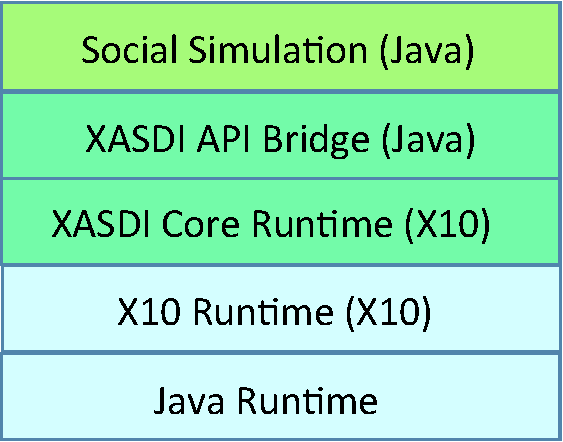
\includegraphics[width=4cm]{Figs.mizuta/xasdistack.pdf}
  \caption{XASDI Software Stack}
  \label{fig:Figs.mizuta/xasdistack}
\end{figure}


The agent in XASDI is referred to as Citizen and Citizen has corresponding CitizenProxy that is managed in the simulation environment to exchange messages.
To manage CitizenProxy, XASDI provides a hierarchical container structure called Place, Region and World (see Figure~\ref{fig:Figs.mizuta/xasdiclass}. CitizenProxies belong to a Place and Places belong to a Region. World can contain several Regions, but usually there is only one Region in the World.


Here, we need to note that the confusing terminology of the X10 programming language and the framework.
The X10 use the term ``Place'', too, but the meaning of the term is different.
The Place of X10 is used to denote the distributed execution environment for multi-core or multi-node.
For this meaning, we will use ``X10 Place (node)'' in distinction from the Place container of agents.
Only one World instance exists in one X10 Place and manages lists of entities in the world including Region and Citizen.
The world can also contain IDs of Citizens in other nodes.

\begin{figure}[h]
  \centering
  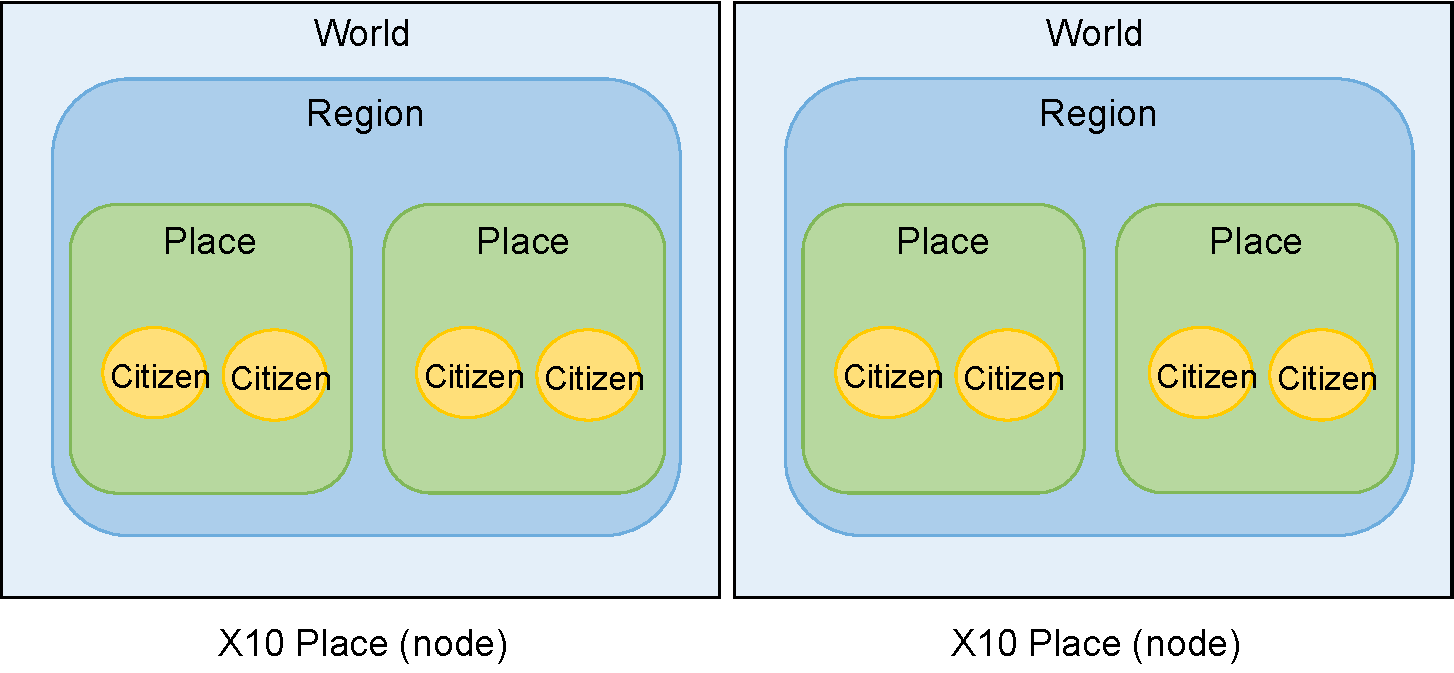
\includegraphics[width=8cm]{Figs.mizuta/xasdiclass.pdf}
  \caption{XASDI hierarchical structure to manage agents}
  \label{fig:Figs.mizuta/xasdiclass}
\end{figure}

Other important classes in XASDI are Message, MessageRepository and Driver.
MessageRepository manages Message exchange among CitizenProxy and environment and this class also works as interface between Java environment and X10 environment to exchange Messages in distributed X10 Places.
Driver manages execution of the simulation with a corresponding thread. Each Driver is related to Places (and Citizens in the Places) where it has a responsibility for execution.

Finally, XASDI provides a logging mechanism. By preparing log definitions for the application, it can output the simulation log at each X10 Places. 


Application users of XASDI need to develop their own simulation application by utilizing these classes and execute the application with XASDI library on Java and X10.
We describe the execution process on XASDI and the simple customization for the sample application bundled with XASDI.

A user starts the simulation by executing the shell script to invoke the X10 core runtime.
After the preparation of X10 environment, Launcher for the simulation written by Java is called at each X10 Place.
Launcher reads the initialization file and generates a Region, Places and Drivers.
If agents are needed to exist from the beginning of the simulation, Launcher or Driver generates Citizens.
Citizens can also be generated by Driver through the method of the Region during the simulation at given time or randomly. For example, consumer agents are generated when they enter a shopping mall.

The main simulation process is executed through Drivers.
Simulation managers in the X10 core environment generate threads and invokes call back method in each Driver in parallel.
One simulation time step can be divided into phases. The number of phases are determined at the beginning of the simulation with initialization file.
The method of the Driver looks at the time and phase given by the environment and determines the action that the corresponding Places and Citizens should perform.


In one node, there is one Region instance that manages the execution of the simulator.
The core framework written using X10 manages the Regions and Message Repositories of distributed nodes.
The Message Repository supports several kinds of messages such as individual message, broadcast message, and control message to move agent between X10 Places.
An individual message is a standard message from one agent to another.
A broadcast message is sent to all nodes and received by the Region or agents corresponding to the type of message.
A move message is a control message for X10 core runtime to remove the Citizen at the source node and restore it at the destination node with serialized field data stored in the message.

MySample application bundled with XASDI demonstrates simple message transactions.
SampleLauncher prepares the simulation by generating a SampleRegion and a SampleDriver.
The SampleDriver generate SampleCitizens at first and executes various type of message transactions by using methods of SampleCitizenProxy or SampleRegion at each time step.
When SampleCitizen receives a message, it records the type and attribute of the message with the logging mechanism provided from the World.

XASDI Development Guide provides a step-by-step description of developing the sample application and debugging it with Eclipse.

Fig.~\ref{fig:Figs.mizuta/xasdiscaling} shows the weak scaling performance of XASDI by using our application for shopping mall simulation with purchasing and walking behavior.
\begin{figure}[h]
  \centering
  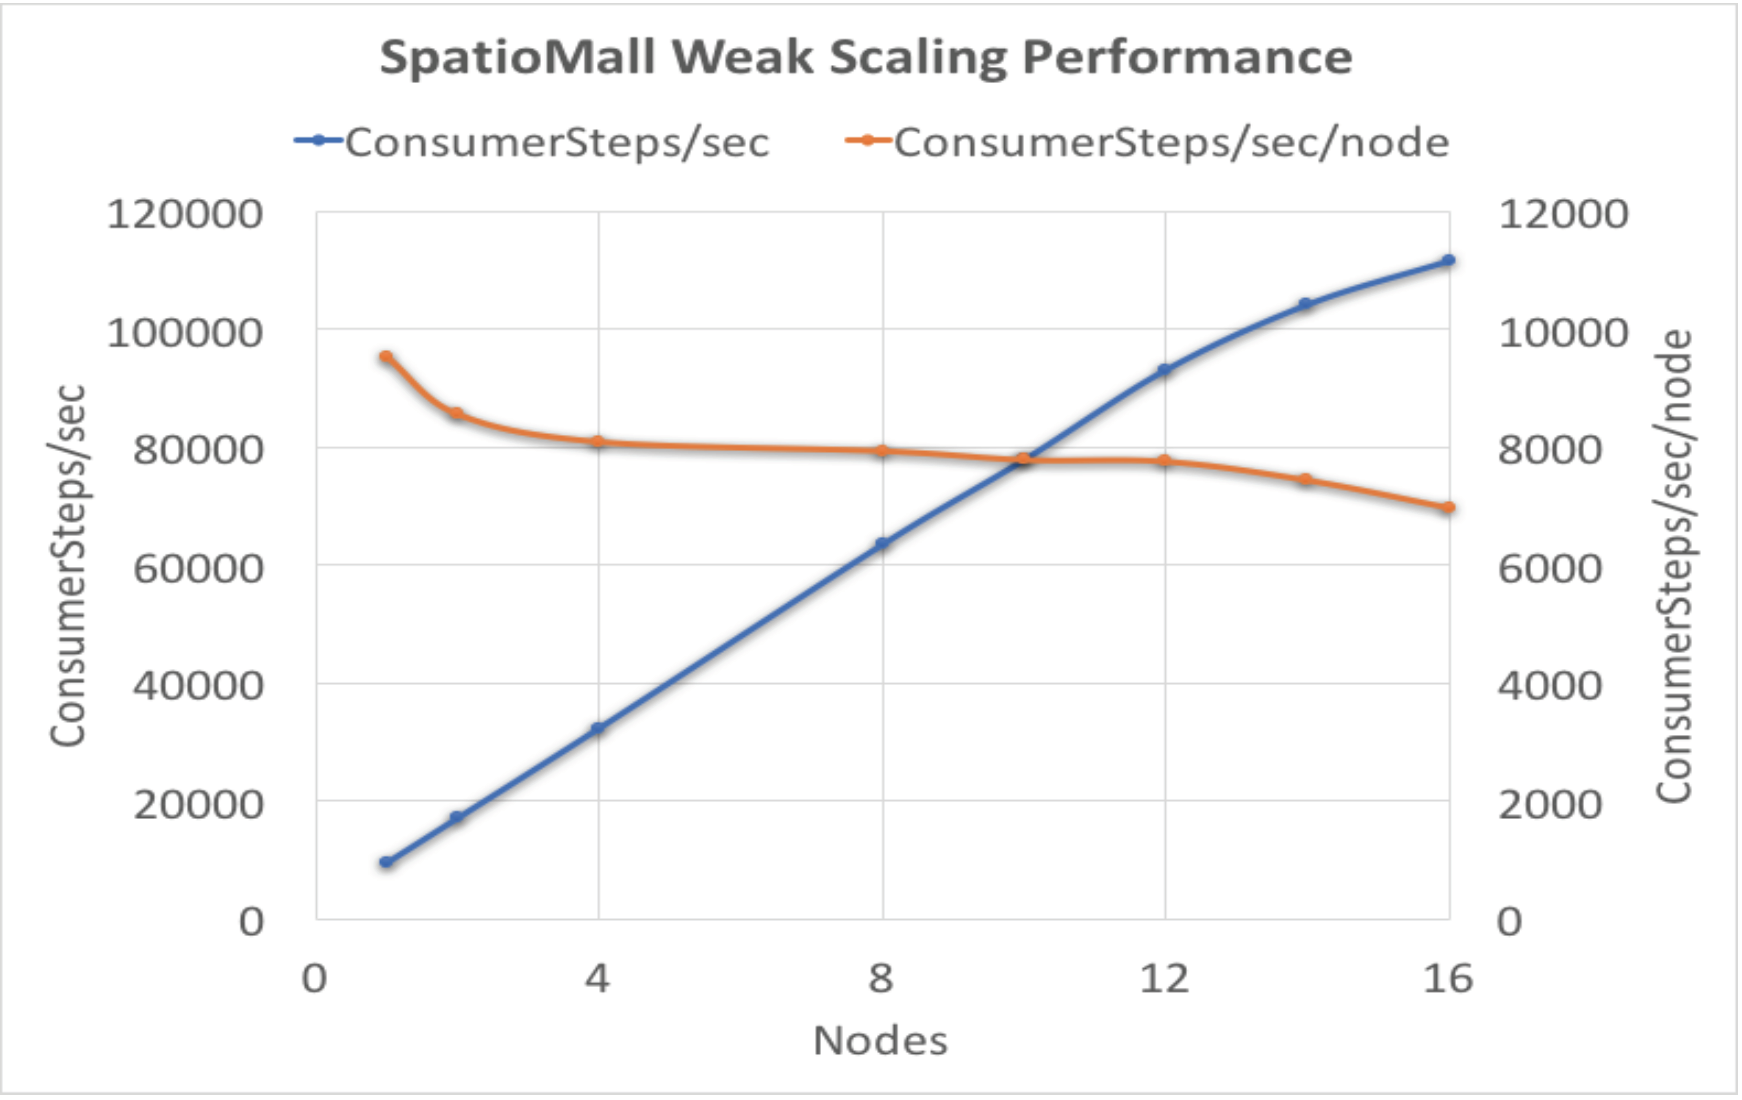
\includegraphics[width=8cm]{Figs.mizuta/xasdiscaling.png}
  \caption{Weal scaling performance of XASDI with shopping mall application.}
  \label{fig:Figs.mizuta/xasdiscaling}
\end{figure}
